\documentclass[a4paper,pra,aps,twocolumn,superscriptaddress,10pt,final]{revtex4-2}
\usepackage[pretty,uselistings]{revquantum}
% \usepackage[brazil]{babel}
\usepackage[T1]{fontenc}
\usepackage[utf8]{inputenc}
\usepackage{stmaryrd} 
\SetSymbolFont{stmry}{bold}{U}{stmry}{m}{n} 
\usepackage{bm}
\usepackage{amsmath}
\usepackage{amssymb}
\usepackage{amsfonts}
\usepackage{silence}
\WarningFilter{revtex4-2}{Repair the float}
\usepackage{anyfontsize}
\usepackage{lipsum}
\usepackage{float}
\usepackage{graphicx}
\usepackage{multirow}
% \usepackage{multicol}
\usepackage{wrapfig}
\usepackage[paperwidth=210mm,paperheight=297mm,centering,hmargin=2cm,vmargin=2.5cm]{geometry}
%=============================================================================
% FRONT MATTER
%=============================================================================

\begin{document}

\title{Atividade prática da disciplina de Matemática Computacional}

\author{Paulo Vinicius Pereira Pinheiro}
\email{paulovpp@gmail.com}
\affiliation{UNINTER - Centro Universitário Internacional}
\affiliation{RU: 3760288}

\date{\today}

\begin{abstract}
    A crescente necessidade por segurança nas transações online traz à tona um problema de grande complexidade: até quando os protocolos atuais de segurança da informação serão capazes de nos manter seguros? Inúmeros são casos de quebra de segurança ou vazamento de dados. Mesmo com uma grande quantidade de métodos utilizados para comunicação segura, não há garantias de plena segurança para nenhum deles. Dentre todos os métodos existentes, destaca-se a criptografia. De forma simétrica ou assimétrica, o ato de criptografar uma mensagem é torná-la inelegível a aqueles à quem a mensagem não se destina. A criptografia é um dos tópicos abordados na disciplina de matemática computacional do curso de engenharia da computação da UNINTER. E o trabalho realizado trata do assunto de forma aplicada. Através da Cifra de Feistel, pode-se compreender com mais clareza os procedimentos de codificação e decodificação de mensagens criptografados. Pra tal, são solicitados os seguintes procedimentos: que sejam codificados os 4 primeiros caracteres do primeiro nome do aluno utilizando-se a cifra simétrica de Feistel com apenas 2 estágios, utilizando o último dígito do RU não nulo, $K$,  como a chave criptográfica para ambos os estágios. Deve-se utilizar também como função $F$ um shift left, cíclico, de $K$ posições. Solicita-se também que a mensagem codificada seja preparada para transmissão e que, em seguida, haja o processo de decodificação, comprovando assim a reciprocidade do processo.
    
    
\end{abstract}

\maketitle

%=============================================================================
% MAIN DOCUMENT
%=============================================================================

\section{Introdução}
\label{sec:intro}

    Criptografia é o processo de codificar ou embaralhar uma mensagem que se deseja transmitir, de tal modo que apenas aquele à quem a mensagem se destine tenha meios para identificar seu conteúdo. Inúmeros são os usos da criptografia para comunicação segura, como em transações financeiras, governamentais e empresariais. 

    Diversos são os métodos criptográficos existentes, cada um com vantagens e desvantagens. No entanto, um ponto há em comum entre eles: todos são passíveis de serem quebrados. Mesmo que se necessite de um tempo exponencialmente grande, ainda sim, haverá uma forma de quebrar esses métodos. A maior promessa contra a criptografia atual é a recém invenção dos computadores quântico. Esses, que possuem um pode computacional muito superior aos computadores atuais, prometem quebrar qualquer método criptográfico em apenas alguns segundos.

    Dentre os métodos criptográficos mais comuns, destaca-se uma divisão em duas grandes categorias: as criptografias de chave simétrica e a assimétrica. A simétrica necessita de apenas uma chave secreta que é responsável por ambos os processos de codificação e decodificação. Nesse caso, ambos os participantes da comunicação necessitam conhecê-la. Nota-se aí o maior gargalo do método pois não há forma perfeitamente segura de transmitir essa chave.
    
    A criptografia de chave assimétrica necessita de duas chaves secretas, uma para cada processo. Duas chaves são produzidas: uma para criptografar e outra para descriptografar as mensagens. A primeira é distribuída publicamente, para todos que desejarem se comunicar possam codificar suas mensagens. A segunda é mantida secreta, pois somente com ela é possível realizar a decodificação.

    O método abordado neste trabalho está categorizado como criptografia de chave simétrica. A Cifra de Feistel, nome dado em honra seu criador, o criptógrafo alemão Horst Feistel, é um método simples e bastante curioso de cifragem pois, se encaixa ainda no modelo de criptografia de blocos, já que é realizada em blocos de tamanho fixo. A figura~\ref{fig:cifra} ilustra a cifragem de forma simplificada.

    \begin{figure}[!htpb]
        \centering
        \label{fig:cifra}
        \caption{Cifra de Feistel.}
        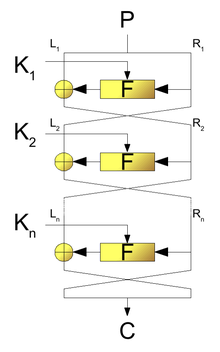
\includegraphics[width=0.25\textwidth]{feistel.png}
        \begin{center}
            \scriptsize{Fonte: \url{https://pt.alegsaonline.com/art/33900}}
        \end{center}
    \end{figure}

    Os processos de codificação e decodificação são idênticos. Eles consistem em dividir a mensagem em dois blocos de tamanhos iguais, aplicar ao segundo bloco uma função \textit{HASH} $F$ de embaralhamento e após, com o primeiro bloco, realizar uma função XOR. A função \textit{HASH}  é gerada a partir de um valor aleatório, conhecido como a chave do processo. Após a função XOR, o resultado é concatenado ao segundo bloco utilizado antes da aplicação da função $F$, que toma a posição inicial no bloco em formação.
    
    Todo esse processo, chamado de iteração, pode ser repetido $n$ vezes, cada um com sua própria chave secreta $k_n$, como mostra a figura~\ref{fig:cifra}. No entanto, para fins de simplificação, este trabalho usará a mesma chave $k$ para as duas iterações.

    A operação de decodificação acontece da mesma forma. As chaves utilizadas nas iterações de decodificação precisam ser as mesmas utilizadas no processo de codificação. Daí decorre sua classificação de cifra de chave simétrica. Portanto, nasce aí o maior problema da cifra de chave simétrica: como compartilhar a chave?
    
    O desenvolvimento deste trabalho, esclarecido na seção~\ref{sec:develop} a seguir, está dividido em duas partes: a subseção~\ref{sec:coding} trata da codificação e a subseção~\ref{sec:decoding} trata da decodificação. Conclusões e considerações finais encontram-se na seção~\ref{sec:conclusion}.

    \section{Desenvolvimento}
    \label{sec:develop}

    Conforme o enunciado do problema, a cifragem deve ocorrer para os primeiros 4 dígitos do nome do aluno. A função $F$ será do tipo \textit{shift left} cíclica, executada $k$ vezes, com $k$ igual ao último dígito não nulo do RU. Este ciclo deve se repetir duas vezes, utilizando a mesma chave para cada iteração.

    Abaixo seguem os processos de codificação e decodificação.

    \subsection{Codificação}
    \label{sec:coding}

    A codificação ocorre conforme elucidação da cifra realizada na introdução~\ref{sec:intro} deste trabalho. Como o primero nome do autor deste trabalho é \textbf{Paulo}, a sequência de caracteres a ser codificada será igual a \textbf{Paul}, com o primeiro caractere "P" maiúsculo. Abaixo, na tabela \ref{tab:tab1-caracteres}, seguem as codificações em decimal e binário, extraídas de uma tabela ASCII para os caracteres selecionados da primeira iteração:

    \begin{table}[!htbp]
        \caption{Conversão dos caracteres a serem codificados.}
        \label{tab:tab1-caracteres}
        \begin{tabular}{|c|c|cl|}
            \hline
            \textbf{Caractere} & \textbf{Decimal} & \multicolumn{2}{c|}{\textbf{Binário}} \\ \hline
            P                  & 80               & \multicolumn{1}{c|}{0101}    & 0000   \\ \hline
            a                  & 97               & \multicolumn{1}{c|}{0110}    & 0001   \\ \hline
            u                  & 117              & \multicolumn{1}{c|}{0111}    & 0101   \\ \hline
            l                  & 108              & \multicolumn{1}{c|}{0110}    & 1100   \\ \hline
        \end{tabular}
    \end{table}

    A tabela \ref{tab:tab1-caracteres} expressa convenientemente cada caractere por seu conjunto de dois \textit{nibbles}, suficientes para proceder com a codificação. Para o segundo \textit{nibble} de cada caractere é executada a função $F$ do tipo \textit{shift left} cíclica oito($8$) vezes, e na sequência o resultado é submetido a uma função $XOR (\oplus)$ com o primeiro nibble. Na tabela \ref{tab:tab2-funcao}, elucida-se os resultados obtidos para cada caractere:

    \begin{table}[!htbp]
        \caption{Funções $F$ e XOR para $1^a$ iteração.}
        \label{tab:tab2-funcao}
        \begin{tabular}{|c|cc|c|c|}
            \hline
            \textbf{Caractere} & \multicolumn{2}{c|}{\textbf{Binário}} & \textbf{Função $F$} & \textbf{XOR ($\oplus$)} \\ \hline
            P                  & \multicolumn{1}{c|}{0101}    & 0000   & 0000                & 0101                                 \\ \hline
            a                  & \multicolumn{1}{c|}{0110}    & 0001   & 0001                & 0111                                 \\ \hline
            u                  & \multicolumn{1}{c|}{0111}    & 0101   & 0101                & 0010                                 \\ \hline
            l                  & \multicolumn{1}{c|}{0110}    & 1100   & 1100                & 1010                                 \\ \hline
        \end{tabular}
    \end{table}

    Para formação da sequência de caracteres codificada, são utilizados dois \textit{nibbles} para cada caractere: o primeiro é obtido do \textit{nibble} prévio à codificação, e o segundo será o resultado da função XOR aplicada, ambos contidos nas colunas 3 e 4 da tabela~\ref{tab:tab2-funcao}. Aplicando a concatenação para todos os caracteres, obtêm-se então a mensagem codificada após uma iteração:

    \begin{table}[!htpb]
        \caption{Mensagem codificada com apenas uma iteração.}
        \label{tab:tab3-iter1}
        \begin{tabular}{|c|}
        \hline
        \textbf{Mensagem extraída da 1$^{\text{a}}$ iteração}  \\ \hline
        0000 0101 0001 0111 0101 0010 1100 1010     \\ \hline
        \end{tabular}%
    \end{table}
    
    A segunda iteração é feita utilizando a mesma chave anterior e com o segundo nibble do caractere obtido da sequência de caracteres codificada da primeira iteração, visualizada na tabela~\ref{tab:tab3-iter1}, segunda linha correspondente aos \textit{nibbles} 2, 4, 6 e 8. A tabela~\ref{tab:tab4-funcao} mostra as aplicações das funções $F$ e XOR para cada caractere da segunda iteração:

    \begin{table}[!htpb]
        \caption{Funções $F$ e XOR para $2^a$ iteração.}
        \label{tab:tab4-funcao}
        \begin{tabular}{|cc|c|c|}
        \hline
        \multicolumn{2}{|c|}{\textbf{Mensagem}} & \textbf{Função $F$} & \textbf{XOR ($\oplus$)} \\ \hline
        \multicolumn{1}{|c|}{0101}    & 0101    & 0101                & 0101                                 \\ \hline
        \multicolumn{1}{|c|}{0110}    & 0111    & 0111                & 0110                                 \\ \hline
        \multicolumn{1}{|c|}{0111}    & 0010    & 0010                & 0111                                 \\ \hline
        \multicolumn{1}{|c|}{0110}    & 1010    & 1010                & 0110                                 \\ \hline
        \end{tabular}
    \end{table}

    A sequência de caracteres codificada após a segunda iteração é dada pela tabela~\ref{tab:tab5-mens}. Essa será a mensagem CODIFICADA que deverá ser transmitida para um destinatário.

    \begin{table}[!htpb]
        \caption{Mensagem codificada após duas iterações.}
        \label{tab:tab5-mens}
        \begin{tabular}{|c|}
        \hline
        \textbf{Mensagem codificada}  \\ \hline
        0101 0101 0110 0111 0111 0010 0110 1010     \\ \hline
        \textbf{V $\qquad\quad$ g $\qquad \quad$ r $\qquad \quad$ j} \\ \hline
        \end{tabular}%
    \end{table}

    A tabela~\ref{tab:tab5-mens} mostra a sequência de caracteres codificada após a segunda iteração, realizando assim a codificação solicitada. Na sequência, o processo de decodificação é desenvolvido.

    \subsection{Decodificação}
    \label{sec:decoding}

    Como prova de conceito, realiza-se agora o processo de decodificação da mensagem previamente codificada. O processo decorre de forma semelhante à codificação, através da aplicação sequenciada das funções $F$ e XOR.
    
    Seguindo o mesmo procedimento da codificação, na primeira iteração da decodificação, o segundo nibble de cada caractere é submetido à função $F$ e em seguida, com o primeiro nibble, a função XOR. Aplicando-se as funções para todos os caracteres, com seus resultados mostrados na tabela~\ref{tab:tab6-funcao}, obtêm-se a sequência de caracteres decodificada mostrada na tabela~\ref{tab:tab7-iter1-deco}.

    \begin{table}[!htpb]
        \caption{Funções $F$ e XOR para $1^a$ iteração da decodificação.}
        \label{tab:tab6-funcao}
        \begin{tabular}{|cc|c|c|}
            \hline
            \multicolumn{2}{|c|}{\textbf{Mensagem}} & \textbf{Função $F$} & \textbf{XOR ($\oplus$)} \\ \hline
            \multicolumn{1}{|c|}{0101}    & 0101    & 0101                & 0000                                 \\ \hline
            \multicolumn{1}{|c|}{0110}    & 0111    & 0111                & 0001                                 \\ \hline
            \multicolumn{1}{|c|}{0111}    & 0010    & 0010                & 0101                                 \\ \hline
            \multicolumn{1}{|c|}{0110}    & 1010    & 1010                & 1100                                 \\ \hline
        \end{tabular}
    \end{table}
    
    \vspace{-0.5cm}
    
    \begin{table}[!htpb]
        \caption{Mensagem decodificada com apenas uma iteração.}
        \label{tab:tab7-iter1-deco}
        \begin{tabular}{|clll|}
        \hline
        \multicolumn{4}{|c|}{\textbf{Mensagem codificada}}            \\ \hline
        \multicolumn{4}{|c|}{0101 0000 0111 0001 0010 0101 1010 1100} \\ \hline
        \end{tabular}%
    \end{table}

    A segunda iteração da decodificação ocorre de forma semelhante a primeira mas sem a inversão dos nibbles ao final da formação dos caracteres. A tabela~\ref{tab:tab8-funcao-deco} mostra os resultados das aplicações das funções $F$ e XOR para cada caractere da segunda iteração:
    
    \vspace{-0.25cm}

    \begin{table}[!htpb]
        \caption{Funções $F$ e XOR para $2^a$ iteração da decodificação.}
        \label{tab:tab8-funcao-deco}
        \begin{tabular}{|cc|c|c|}
            \hline
            \multicolumn{2}{|c|}{\textbf{Mensagem}} & \textbf{Função $F$} & \textbf{XOR (\textbackslash{}oplus)} \\ \hline
            \multicolumn{1}{|c|}{0101}    & 0000    & 0101                & 0101                                 \\ \hline
            \multicolumn{1}{|c|}{0110}    & 0001    & 0111                & 0110                                 \\ \hline
            \multicolumn{1}{|c|}{0111}    & 0101    & 0010                & 0111                                 \\ \hline
            \multicolumn{1}{|c|}{0110}    & 1100    & 1100                & 0110                                 \\ \hline
            \end{tabular}
    \end{table}

    A formação do byte correspondente a cada caractere é realizada sem a inversão dos nibbles ao final das operações. A tabela~\ref{tab:tab9-mens-deco} mostra os resultados das concatenações utilizadas para composição dos caracteres da mensagem final decodificada.

    \begin{table}[!htpb]
        \caption{Mensagem decodificada.}
        \label{tab:tab9-mens-deco}
        \begin{tabular}{|c|}
            \hline
            \textbf{Mensagem codificada}                      \\ \hline
            0101 0000 0110 0001 0111 0101 0110 1100           \\ \hline
            \textbf{P $\qquad \quad \quad$ a $\quad \qquad$ u $\qquad \quad \quad$ l} \\ \hline
        \end{tabular}%
    \end{table}

\section{Conclusão}
\label{sec:conclusion}
    
    Neste trabalho foram realizadas a codificação e decodificação de uma mensagem pela Cifra de Feister, um modelo de criptografia de chave simétrica e de bloco geralmente utilizada com 64 bits. A mensagem original foi determinada a partir dos primeiros quatro caracteres do primeiro nome do autor. A função $F$ solicitada como foi a \textit{shift left} cíclico pelo número de vezes correspondente ao último dígito não inteiro do RU. E o número de interações solicitado para cada processo foi de duas iterações com a mesma chave cada.
    
    A seção de desenvolvimento foi dividida em duas partes, para os processos de codificação e decodificação correspondentemente. Tabelas foram apresentadas com o passos intermediários e os resultados preliminares das operações. As mensagens codificada e decodificada podem ser encontradas correspondentemente nas tabelas~\ref{tab:tab5-mens} e~\ref{tab:tab9-mens-deco}. Os resultados estão de acordo com o solicitado no enunciado do trabalho.

    Conclui-se também que a Cifra de César possui um baixo custo de processamento para codificação e decodificação, já que é realizada em bloco. Porém, como trata-se de uma cifra simétrica, o problema de  compartilhamento da chave ainda permanece. Espera-se que o problema de compartilhamento de chaves privadas possa ser resolvido na computação clássica como já é trabalhado na computação quântica.

    \vspace{-0.5cm}

    \begin{acknowledgments}
        O autor agradece aos professores, tutores e a todo pessoal responsável pela disciplina de matemática computacional pela oportunidade de produzir tal trabalho que sem dúvida, aprofundou o conhecimento adquirido no período de estudos.

        O autor deseja também um esclarecimento por parte dos professores/tutores da disciplina, que pode ser fornecido naturalmente por e-mail: pelo explanado na aula 06, a cifra deveria ter sido realizada em todo o bloco formado pelos quatro caracteres, compondo um total de quatro bytes ou 32 bits. Entretanto, conforme aula ao vivo, realizada no dia 19 de maio às 19h30 fora explanada a cifra realizada individualmente por cada caractere. O esclarecimento seria sobre a utilização das duas formas. E se alguma forma é mais eficiente/segura que a outra, se realizando as iterações por bloco de caracteres ou individualmente.

        Trabalho realizado em \LaTeX.
    \end{acknowledgments}
% \bibliography{example}

%=============================================================================
% APPENDICES
%=============================================================================

\appendix

% %=============================================================================
\section{Processo de codificação}
\label{apx:code}

    Abaixo segue uma imagem do processo de codificação e decodificação da mensagem solicitada usando a Cifra de Feister.

\onecolumngrid

    \begin{figure*}[!htpb]
        \centering
        \caption{Imagem retirada do microsoft excel com o processamento da cifra solicitada.}
        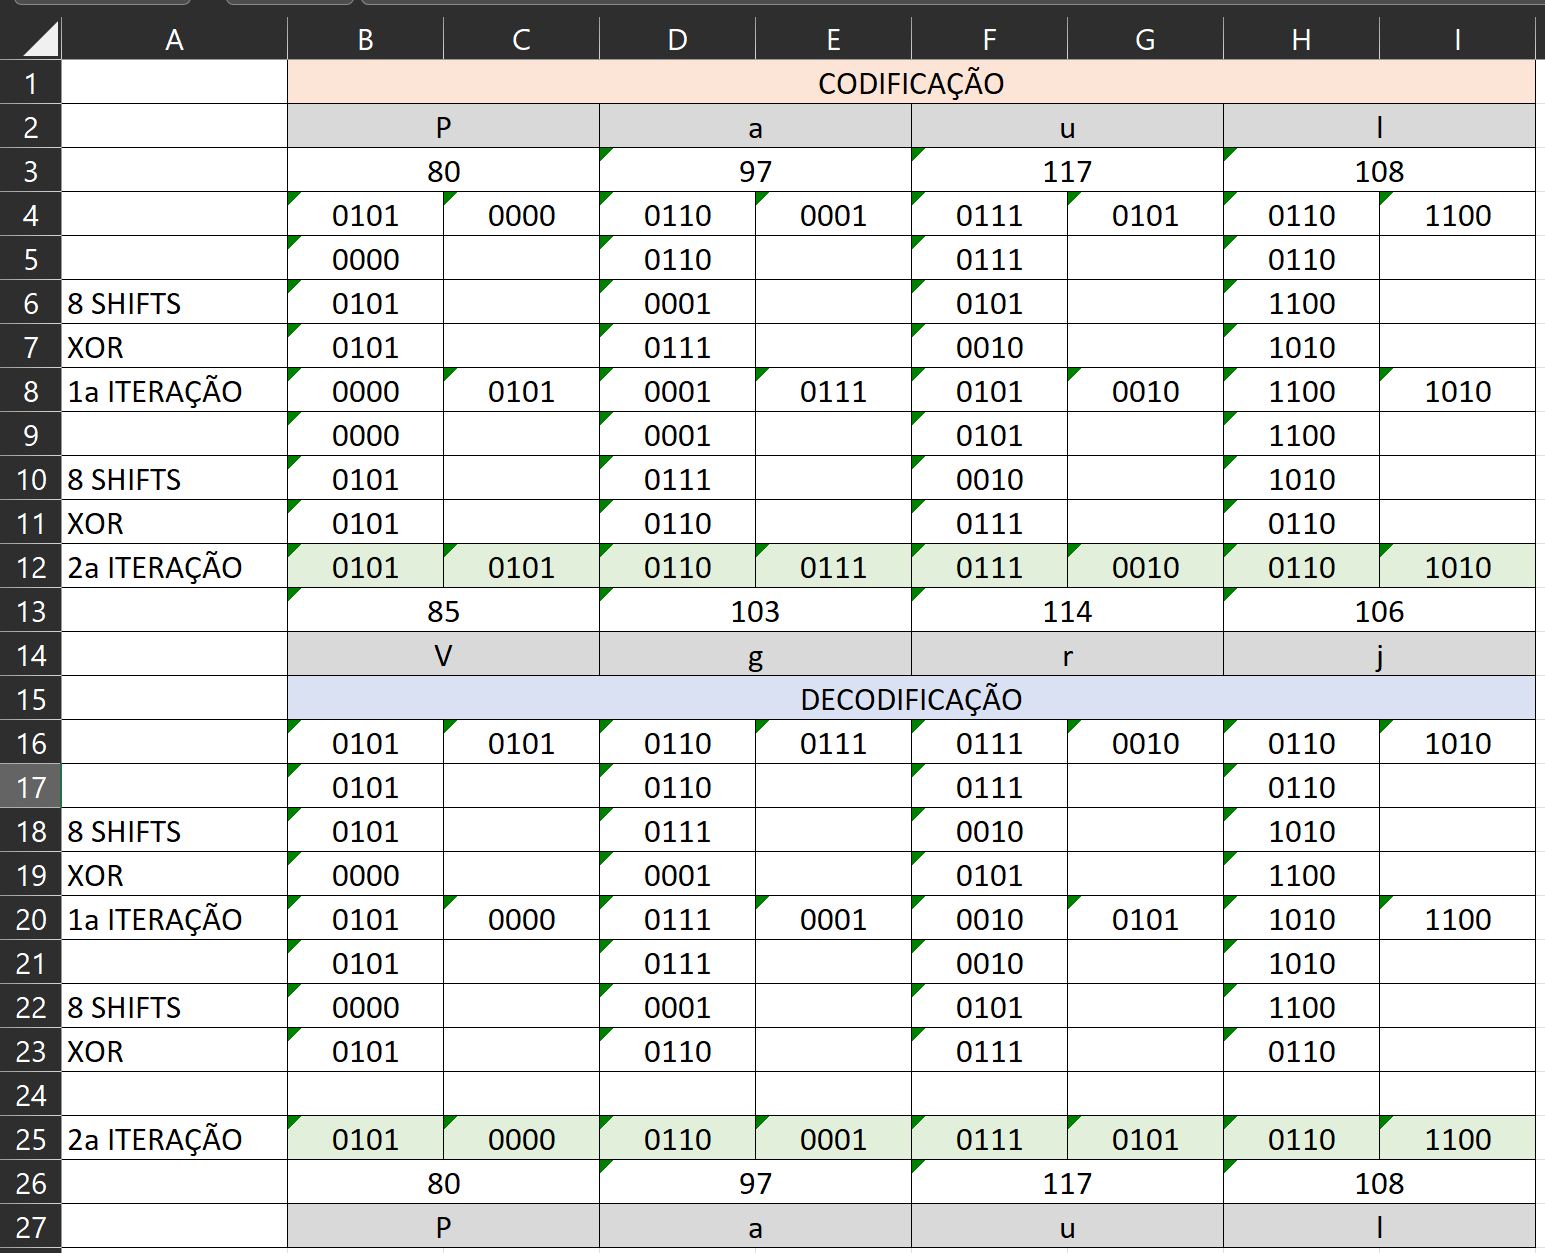
\includegraphics[width=\textwidth]{Tabela-cifra.png}
        \label{fig:Tabela-cifra}
    \end{figure*}

\end{document} 